% Options for packages loaded elsewhere
% Options for packages loaded elsewhere
\PassOptionsToPackage{unicode}{hyperref}
\PassOptionsToPackage{hyphens}{url}
\PassOptionsToPackage{dvipsnames,svgnames,x11names}{xcolor}
%
\documentclass[
  indonesian,
]{article}
\usepackage{xcolor}
\usepackage{amsmath,amssymb}
\setcounter{secnumdepth}{-\maxdimen} % remove section numbering
\usepackage{iftex}
\ifPDFTeX
  \usepackage[T1]{fontenc}
  \usepackage[utf8]{inputenc}
  \usepackage{textcomp} % provide euro and other symbols
\else % if luatex or xetex
  \usepackage{unicode-math} % this also loads fontspec
  \defaultfontfeatures{Scale=MatchLowercase}
  \defaultfontfeatures[\rmfamily]{Ligatures=TeX,Scale=1}
\fi
\usepackage{lmodern}
\ifPDFTeX\else
  % xetex/luatex font selection
\fi
% Use upquote if available, for straight quotes in verbatim environments
\IfFileExists{upquote.sty}{\usepackage{upquote}}{}
\IfFileExists{microtype.sty}{% use microtype if available
  \usepackage[]{microtype}
  \UseMicrotypeSet[protrusion]{basicmath} % disable protrusion for tt fonts
}{}
\makeatletter
\@ifundefined{KOMAClassName}{% if non-KOMA class
  \IfFileExists{parskip.sty}{%
    \usepackage{parskip}
  }{% else
    \setlength{\parindent}{0pt}
    \setlength{\parskip}{6pt plus 2pt minus 1pt}}
}{% if KOMA class
  \KOMAoptions{parskip=half}}
\makeatother
% Make \paragraph and \subparagraph free-standing
\makeatletter
\ifx\paragraph\undefined\else
  \let\oldparagraph\paragraph
  \renewcommand{\paragraph}{
    \@ifstar
      \xxxParagraphStar
      \xxxParagraphNoStar
  }
  \newcommand{\xxxParagraphStar}[1]{\oldparagraph*{#1}\mbox{}}
  \newcommand{\xxxParagraphNoStar}[1]{\oldparagraph{#1}\mbox{}}
\fi
\ifx\subparagraph\undefined\else
  \let\oldsubparagraph\subparagraph
  \renewcommand{\subparagraph}{
    \@ifstar
      \xxxSubParagraphStar
      \xxxSubParagraphNoStar
  }
  \newcommand{\xxxSubParagraphStar}[1]{\oldsubparagraph*{#1}\mbox{}}
  \newcommand{\xxxSubParagraphNoStar}[1]{\oldsubparagraph{#1}\mbox{}}
\fi
\makeatother


\usepackage{longtable,booktabs,array}
\newcounter{none} % for unnumbered tables
\usepackage{calc} % for calculating minipage widths
% Correct order of tables after \paragraph or \subparagraph
\usepackage{etoolbox}
\makeatletter
\patchcmd\longtable{\par}{\if@noskipsec\mbox{}\fi\par}{}{}
\makeatother
% Allow footnotes in longtable head/foot
\IfFileExists{footnotehyper.sty}{\usepackage{footnotehyper}}{\usepackage{footnote}}
\makesavenoteenv{longtable}
\usepackage{graphicx}
\makeatletter
\newsavebox\pandoc@box
\newcommand*\pandocbounded[1]{% scales image to fit in text height/width
  \sbox\pandoc@box{#1}%
  \Gscale@div\@tempa{\textheight}{\dimexpr\ht\pandoc@box+\dp\pandoc@box\relax}%
  \Gscale@div\@tempb{\linewidth}{\wd\pandoc@box}%
  \ifdim\@tempb\p@<\@tempa\p@\let\@tempa\@tempb\fi% select the smaller of both
  \ifdim\@tempa\p@<\p@\scalebox{\@tempa}{\usebox\pandoc@box}%
  \else\usebox{\pandoc@box}%
  \fi%
}
% Set default figure placement to htbp
\def\fps@figure{htbp}
\makeatother



\ifLuaTeX
\usepackage[bidi=basic,shorthands=off,provide=*]{babel}
\else
\usepackage[bidi=default,shorthands=off,provide=*]{babel}
\fi
\ifLuaTeX
  \usepackage{selnolig} % disable illegal ligatures
\fi


\setlength{\emergencystretch}{3em} % prevent overfull lines

\providecommand{\tightlist}{%
  \setlength{\itemsep}{0pt}\setlength{\parskip}{0pt}}



 


\let\maketitle\relax
\makeatletter
\@ifpackageloaded{caption}{}{\usepackage{caption}}
\AtBeginDocument{%
\ifdefined\contentsname
  \renewcommand*\contentsname{Daftar Isi}
\else
  \newcommand\contentsname{Daftar Isi}
\fi
\ifdefined\listfigurename
  \renewcommand*\listfigurename{Daftar Gambar}
\else
  \newcommand\listfigurename{Daftar Gambar}
\fi
\ifdefined\listtablename
  \renewcommand*\listtablename{Daftar Tabel}
\else
  \newcommand\listtablename{Daftar Tabel}
\fi
\ifdefined\figurename
  \renewcommand*\figurename{Gambar}
\else
  \newcommand\figurename{Gambar}
\fi
\ifdefined\tablename
  \renewcommand*\tablename{Tabel}
\else
  \newcommand\tablename{Tabel}
\fi
}
\@ifpackageloaded{float}{}{\usepackage{float}}
\floatstyle{ruled}
\@ifundefined{c@chapter}{\newfloat{codelisting}{h}{lop}}{\newfloat{codelisting}{h}{lop}[chapter]}
\floatname{codelisting}{Daftar}
\newcommand*\listoflistings{\listof{codelisting}{Daftar Daftar}}
\makeatother
\makeatletter
\makeatother
\makeatletter
\@ifpackageloaded{caption}{}{\usepackage{caption}}
\@ifpackageloaded{subcaption}{}{\usepackage{subcaption}}
\makeatother
\usepackage{bookmark}
\IfFileExists{xurl.sty}{\usepackage{xurl}}{} % add URL line breaks if available
\urlstyle{same}
\hypersetup{
  pdftitle={Uji Coba Automasi Laporan Quarto dengan RStudio},
  pdfauthor={Bimasuci Basiludin},
  pdflang={id},
  colorlinks=true,
  linkcolor={blue},
  filecolor={Maroon},
  citecolor={Blue},
  urlcolor={Blue},
  pdfcreator={LaTeX via pandoc}}


\title{Uji Coba Automasi Laporan Quarto dengan RStudio}
\author{Bimasuci Basiludin}
\date{2026-07-23}
\begin{document}
\maketitle

\begin{titlepage}
  \definecolor{coverblue}{HTML}{004488}
  \definecolor{goldline}{HTML}{FFD700}
  \pagecolor{coverblue} % Mewarnai latar belakang cover menjadi biru
  \thispagestyle{empty} % Menghilangkan nomor halaman pada cover

  \centering
  \vspace*{0cm}

  % Memasukkan Logo (Pastikan file logo-nobg.png ada di folder yang sama)
  
\includegraphics[width=4.5cm]{logo-nobg.png}\par\vspace{3cm}

  % Judul Laporan
  {\huge\bfseries\color{white} Uji Coba Automasi Laporan Quarto dengan RStudio \par}
  \vspace{0.5cm}

  % Garis Dekorasi Emas
  {\color{goldline}\hrule height 2pt}\par
  \vspace{1.5cm}

  % Nama Penulis
  {\Large\bfseries\color{white} Bimasuci Basiludin \par}

  \vfill
  % Tanggal di bagian bawah
  {\large\color{white} \today \par}
\end{titlepage}
\nopagecolor % Mengembalikan warna halaman berikutnya menjadi putih standar

\renewcommand*\contentsname{Daftar Isi}
{
\setcounter{tocdepth}{3}
\tableofcontents
}

\clearpage

\subsection{1. Menampilkan 5 data
teratas}\label{menampilkan-5-data-teratas}

Pertama, kita akan mencoba untuk menampilkan sampel 5 data teratas dari
sumber data yang digunakan.

\begin{figure}[H]

{\centering \pandocbounded{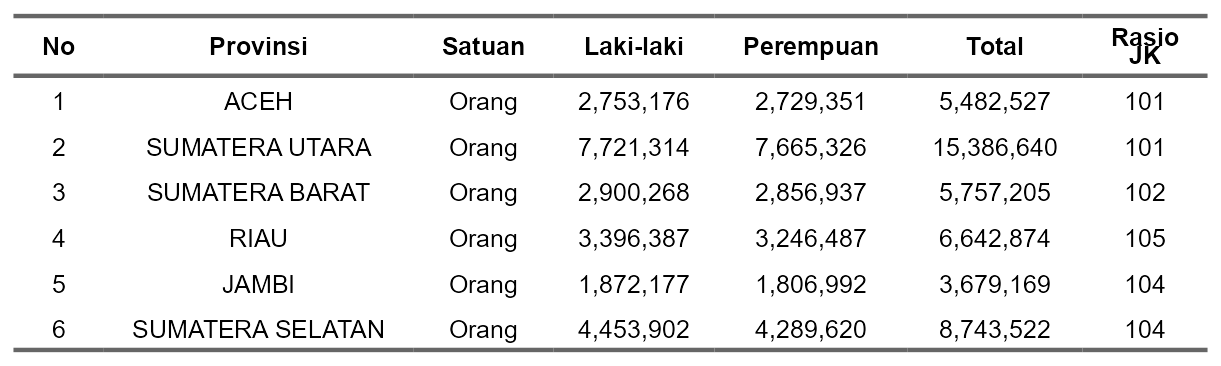
\includegraphics[keepaspectratio]{tabel_5_teratas.png}}

}

\caption{Lima Data Pertama Dataset Kependudukan Indonesia 2023}

\end{figure}%

\subsection{2. Merapihkan nama kolom dan mengurutkan berdasarkan total
penduduk}\label{merapihkan-nama-kolom-dan-mengurutkan-berdasarkan-total-penduduk}

Kemudian kita rapihkan nama kolom dan menampilkannya kembali secara utuh
dengan mengurutkannya berdasarkan total penduduk.

\begin{figure}[H]

{\centering \pandocbounded{
\includegraphics[keepaspectratio]{tabel_urutan_total.png}}

}

\caption{Data Bersih Kependudukan Indonesia 2023}

\end{figure}%

\subsection{3. Menampilkan Grafik Rasio Jenis Kelamin per
Provinsi}\label{menampilkan-grafik-rasio-jenis-kelamin-per-provinsi}

Selanjutnya kita tampilkan grafik rasio jenis kelamin dari setiap
provinsi.

\begin{figure}[H]

{\centering \pandocbounded{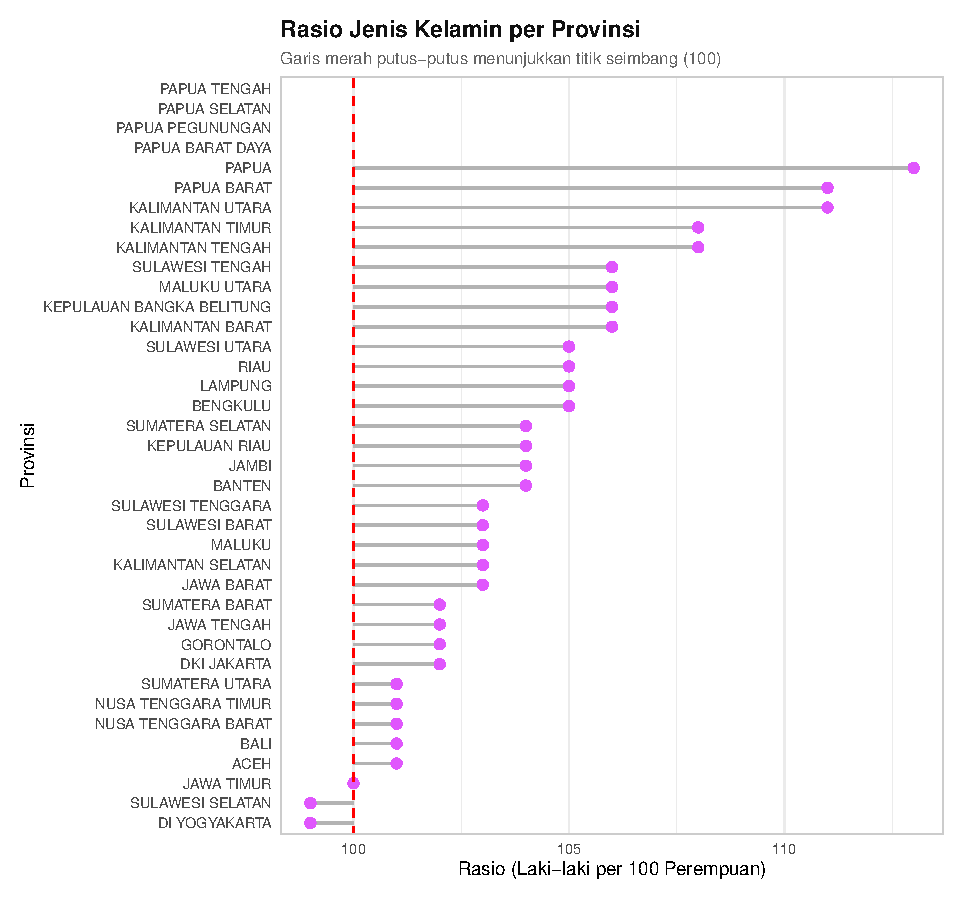
\includegraphics[keepaspectratio]{coba_laporan_files/figure-pdf/unnamed-chunk-4-1.pdf}}

}

\caption{Distribusi Rasio Jenis Kelamin per Provinsi Tahun 2023}

\end{figure}%

\subsection{4. Menampilkan 10 Provinsi dengan Penduduk
Terbanyak}\label{menampilkan-10-provinsi-dengan-penduduk-terbanyak}

Lalu kita tampilkan barchart untuk membandingkan jumlah penduduk dari 10
provinsi dengan jumlah penduduk terbanyak di Indonesia.

\begin{figure}[H]

{\centering \pandocbounded{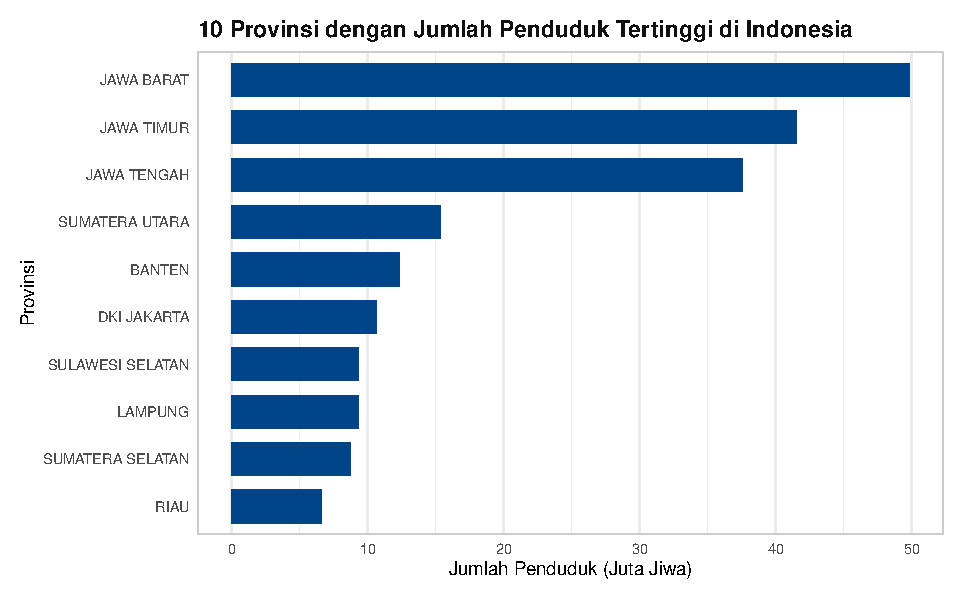
\includegraphics[keepaspectratio]{coba_laporan_files/figure-pdf/unnamed-chunk-5-1.pdf}}

}

\caption{Sepuluh Provinsi dengan Jumlah Penduduk Tertinggi}

\end{figure}%




\end{document}
